\documentclass[tikz,border=2pt]{standalone}
\usepackage{amsmath,amssymb}
\usepackage{tikz}
\usetikzlibrary{arrows.meta}

\begin{document}
% [0,1] has a maximum (1 belongs to the set); (0,1) has no maximum, only the supremum 1.
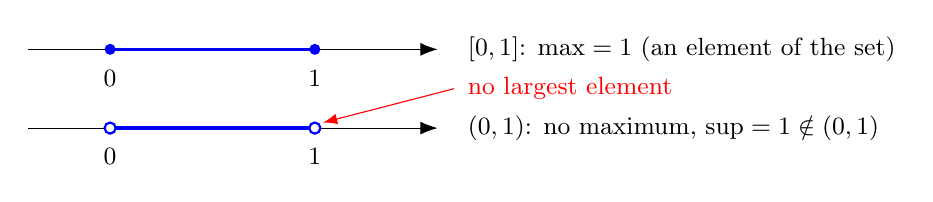
\begin{tikzpicture}[x=2.6cm, every node/.style={font=\small}]
	\draw[-{Latex[length=2.2mm]}] (-0.4,1) -- (1.6,1);
	\draw[very thick, blue] (0,1) -- (1,1);
	\fill[blue] (0,1) circle (2pt); \fill[blue] (1,1) circle (2pt);
	\node[below=4pt] at (0,1) {$0$}; \node[below=4pt] at (1,1) {$1$};
	\node[anchor=west] at (1.7,1) {$[0,1]$: $\max=1$ (an element of the set)};
	\draw[-{Latex[length=2.2mm]}] (-0.4,0) -- (1.6,0);
	\draw[very thick, blue] (0,0) -- (1,0);
	\draw[blue, thick, fill=white] (0,0) circle (2pt); \draw[blue, thick, fill=white] (1,0) circle (2pt);
	\node[below=4pt] at (0,0) {$0$}; \node[below=4pt] at (1,0) {$1$};
	\node[anchor=west] at (1.7,0) {$(0,1)$: no maximum, $\sup=1\notin(0,1)$};
	\draw[-{Latex[length=1.8mm]}, red] (1.68,0.5) -- (1.04,0.07);
	\node[red, anchor=west] at (1.7,0.5) {no largest element};
\end{tikzpicture}
\end{document}
